%% ------------------------------------------------------------------- %%
%% ------------------------------------------------------------------- %%
%% ------------------------------------------------------------------- %%
%% ------------------------------------------------------------------- %%
\chapter{Propuesta}
\label{cap:propuesta}

\lhead{\emph{Propuesta}} 
%% ------------------------------------------------------------------- %%
%% ------------------------------------------------------------------- %%
%% ------------------------------------------------------------------- %%
%% ------------------------------------------------------------------- %%
%% ------------------------------------------------------------------- %%
%% ------------------------------------------------------------------- %%

%% -------------------------------------------------------------------- %%
%% -------------------------------------------------------------------- %%


La detección de neoantígenos es un proceso largo, descrito anteriormente. Debido a esto, esta investigación se ha centrado en la predicción de la unión pMHC, porque es una de las etapas con mayor investigación en el estado del arte y sin embargo, los resultados aún carecen de buen desempeño. En resumen, en este trabajo hemos realizado \textit{fine-tuning} a modelos \textit{Transformer}, para la tarea de predicción de la unión pMHC.




\begin{comment}
	

\section{Predicción de la afinidad peptido-MHC (peptide-MHC binding)}

La propuesta se inspira en los trabajos de \cite{cheng2021bertmhc} y \cite{hashemi2022improved}. Ambos proponen el uso de \textit{transfer  learning} a partir de los modelos pre-entrenados BERT \citep{devlin2018bert} y ESM-1b \citep{rives2021biological} respectivamente. \\


El modelo \textit{Bidirectional Encoder Representations from Transformers.} (BERT), fue diseñado para el pre-entrenamiento de representaciones bidireccionales de textos no etiquetados. Este modelo fue diseñado inicialmente para el procesamiento natural del lenguaje, pero en el trabajo de \cite{rao2019evaluating}, se planteó su uso para secuencias de aminoácidos. Es así que \cite{rao2019evaluating} entrenan BERT con 31 millones de secuencias de proteínas y llaman a su propuesta \textit{Tasks Assessing Protein Embeddings} (TAPE).\\

Recientemente, Facebook desarrolla el modelo ESM-1b \citep{rives2021biological}. La propuesta se basa en el modelo RoBERTa \citep{liu2019roberta}, la cuál es una optimización de BERT. Luego, ESM-1b fue entrenado con la base de datos Uniref50 \citep{suzek2015uniref}, esta base de datos cuenta con aproximadamente 250 millones de secuencias de proteínas. En este caso, se realizó un entrenamiento no supervisado, se ocultaron las etiquetas referentes a la estructura o función de las proteínas.\\

Entonces, la propuesta de la tesis se basa en utilizar \textit{transfer learning} del modelo pre-entrenado ESM-1b, luego se va a utilizar otra red neuronal paralela que se alimente de datos físico-químicos de los aminoácidos. Se propone utilizar las propiedades físico-químicas de los aminoácidos, porque en varios ensayos clínicos se ha comprobado que influyen en la predicción \textit{peptide-MHC binding} y \textit{pMHC-TCR presentation} \citep{gopanenko2020main, borden2022cancer}. Luego, las dos redes neuronales paralelas se unirán en una red neuronal totalmente conectada (ver Figura \ref{fig:proposal}). El objetivo, es aprovechar las propiedades físico-químicas de los aminoácidos para mejorar la afinidad \textit{peptide-MHC}.

Para los entrenamientos y experimentos se utilizará la base de datos HLA3D \citep{li2022hla3d}, esta contiene información de 1296 aminoácidos. Luego, también utilizaremos las muestras recolectadas de \cite{hashemi2022improved}.
\end{comment}

\section{Metodología}

Esta investigación se  enfoca en la tarea de predecir la unión pMHC, descrito en la etapa 3.1 del proceso general para generar vacunas personalizadas basadas en neoantígenos (ver Figura \ref{fig:proposal}). Se ha evaluado  seis modelos \textit{Transformer}s pre-entrenados en diversas tareas de Proteómica como: predicción de estructura de proteínas, predicción de la función de proteínas, etc. Los modelos \textit{Transformer} son: TAPE \citep{rao2019evaluating}, ProtBert-BFD \citep{elnaggar2021prottrans} y ESM2 \citep{lin2023evolutionary} (ESM2(t6), ESM2(t12), ESM2(t30), ESM2(t33)). Durante la evaluación se realizó \textit{fine-tuning} a los modelos agregando un bloque de BiLSTM al final, de igual forma que lo realizó HLAB \citep{zhang2022hlab}. También se evaluó el uso de \textit{Gradient Accumulation Steps} (GAS) y el uso de una metodología para congelar las capas del modelo \textit{Transformer}. En la Figura \ref{fig:proposal}, describimos la propuesta: primero tomamos como entrada el péptido y el MHC, luego estos son concatenados y son recibidos por el modelo \textit{Transformer} y el bloque BiLSTM respectivamente para predecir su afinidad o unión.




\begin{figure}[H]
	\centering
	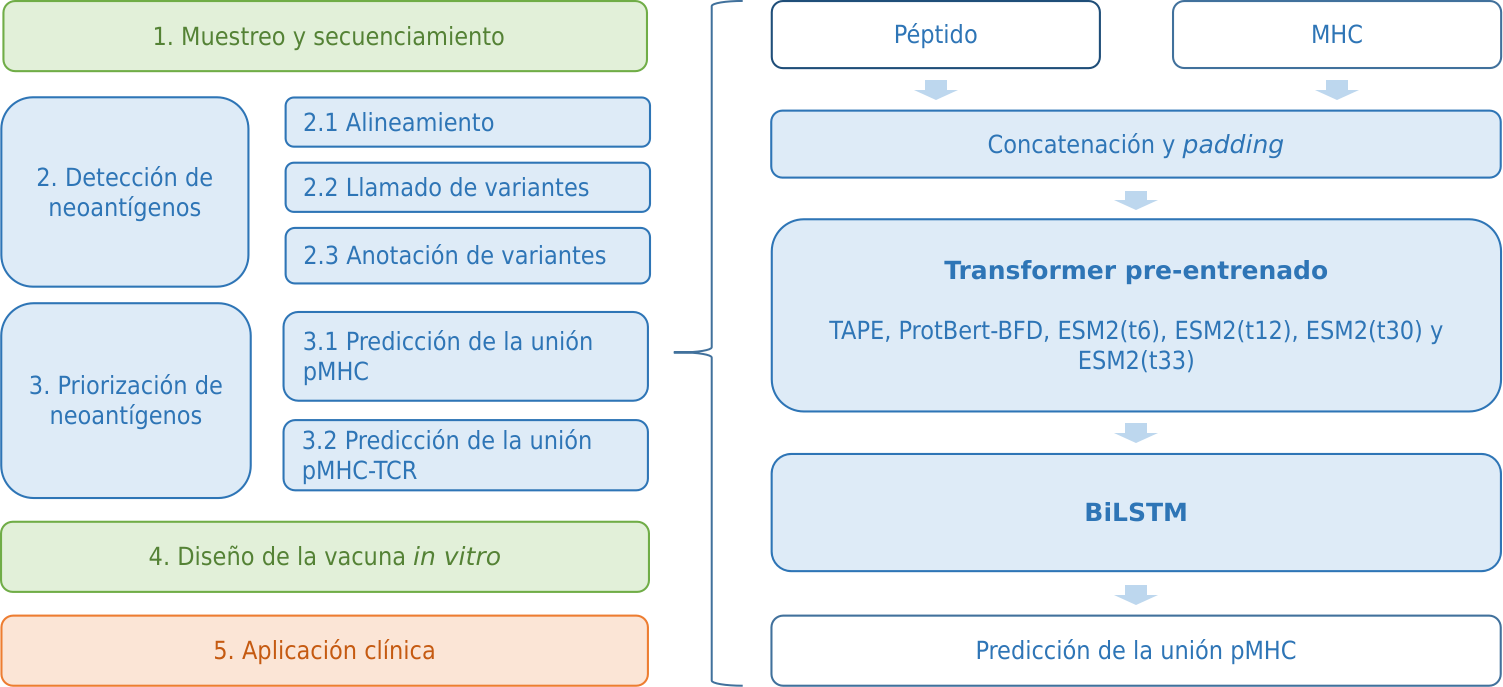
\includegraphics[width=\textwidth]{img/proposal/proposal}	
	\caption{Propuesta de \textit{transfer learning} de ESM-1b y una red neuronal paralela para la predicción de la afinidad entre un péptido y MHC (peptide MHC binding).}
	\label{fig:proposal}
\end{figure}


\section{Bases de datos}
Utilizamos secuencias de péptidos del conjunto de datos Anthem \citep{mei2021anthem}. Este conjunto de datos consta de 539,019 muestras para entrenamiento, 179,673 para validación y 172,580 para pruebas. Por ejemplo, en la Tabla \ref{tab:db_samples}, mostramos algunas muestras de esta base de datos. La columna MHC especifica el tipo de MHC o HLA, luego la columna pseudosecuencia, representa la secuencia de aminoácidos del MHC; esta pseudosecuencia fue obtenida de la base de datos de NetMHCpan4.1. Seguidamente, prosigue la secuencia de aminoácidos del péptido. Finalmente, la ultima columna es la clase o etiqueta, tendrá un valor de uno cuando existe una unión entre el pMHC y cero en caso contrario.


Adicionalmente, en la Figura \ref{fig:samples}, presentamos la distribución de las muestras por \textit{k-mers}. En Bioinformática, se hace referencia al termino \textit{k-mer} para representar secuencias biológicas de ADN, ARN o proteínas. Para el caso específico de proteínas, una secuencia de \textit{8-mer}, defina que la proteína en cuestión esta compuesta por 8 aminoácidos. Para la base de datos utilizada en esta investigación, los péptidos de \textit{9-mers} constituyen la mayoría de las muestras; miesntras que los péoptidos \textit{14-mer} son los mas escazos. Además, estos péptidos \textit{14-mer}, usualmente presentan comportamientos distintos. Esto ha ocasionado que los umbrales utilizados por los clasificadores varia dependiendo del \textit{k-mer} y por tipo de clasificador. 




\begin{table}[H]
	\caption[Ejemplo de algunas muestras de la base de datos]{Ejemplo de algunas muestras de la base de datos. Cada MHC es representado por una pseudosecuencia procesadas por NetMHCpan4.1. Luego los péptidos son cadenas de aminoácidos entreo 8 a 14 amino ácidos. La clase o etiqueta es un cero si existe una unión entre el péptido y el MHC o cero en caso contrario.}
	\label{tab:db_samples}
	\scriptsize
	\setlength{\tabcolsep}{0.5em} % for the horizontal padding
	{\renewcommand{\arraystretch}{1.5}% for the vertical padding
	\begin{tabular}{llll}
		\hline
		\textbf{MHC}         & \textbf{Pseudosecuencia del MHC}                & \textbf{Péptido}        & \textbf{Clase} \\ \hline
		HLA-A*01:01 & YFAMYQENMAHTDANTLYIIYRDYTWVARVYRGY & LFGRDLSY       & 1     \\
		HLA-A*01:01 & YFAMYQENMAHTDANTLYIIYRDYTWVARVYRGY & TDKKTHLY       & 1     \\
		HLA-A*01:01 & YFAMYQENMAHTDANTLYIIYRDYTWVARVYRGY & RSDTPLIY       & 1     \\
		HLA-A*01:01 & YFAMYQENMAHTDANTLYIIYRDYTWVARVYRGY & NSDLVQKY       & 1     \\
		HLA-A*01:01 & YFAMYQENMAHTDANTLYIIYRDYTWVARVYRGY & LSDLLDWK       & 1     \\
		HLA-A*01:01 & YFAMYQENMAHTDANTLYIIYRDYTWVARVYRGY & LLQNDGFF       & 1     \\
		HLA-A*01:01 & YFAMYQENMAHTDANTLYIIYRDYTWVARVYRGY & DSDMQTLV       & 1     \\
		HLA-A*01:01 & YFAMYQENMAHTDANTLYIIYRDYTWVARVYRGY & TDYHVRVY       & 1     \\
		HLA-A*01:01 & YFAMYQENMAHTDANTLYIIYRDYTWVARVYRGY & VLDSEGYL       & 1     \\
		HLA-A*01:01 & YFAMYQENMAHTDANTLYIIYRDYTWVARVYRGY & SDFHNNRY       & 1     \\
		HLA-C*06:02 & YDSGYREKYRQADVNKLYLWYDSYTWAEWAYTWY & FDGRVVTRSYLEKQ & 0     \\
		HLA-C*06:02 & YDSGYREKYRQADVNKLYLWYDSYTWAEWAYTWY & KPCCPDIDIFVDGK & 0     \\
		HLA-C*06:02 & YDSGYREKYRQADVNKLYLWYDSYTWAEWAYTWY & QDLKDFMRQAGEVT & 0     \\
		HLA-C*06:02 & YDSGYREKYRQADVNKLYLWYDSYTWAEWAYTWY & EGYPKSKKQFFEEV & 0     \\
		HLA-C*06:02 & YDSGYREKYRQADVNKLYLWYDSYTWAEWAYTWY & GNHISALKRRYTRR & 0     \\
		HLA-C*06:02 & YDSGYREKYRQADVNKLYLWYDSYTWAEWAYTWY & RHLRTHTGEKPYVC & 0     \\
		HLA-C*06:02 & YDSGYREKYRQADVNKLYLWYDSYTWAEWAYTWY & RGLNGGITPLNSIS & 0     \\
		HLA-C*06:02 & YDSGYREKYRQADVNKLYLWYDSYTWAEWAYTWY & SDFALKNPFYSLEM & 0     \\
		HLA-C*06:02 & YDSGYREKYRQADVNKLYLWYDSYTWAEWAYTWY & ALDSGDASPGTWSG & 0     \\
		HLA-C*06:02 & YDSGYREKYRQADVNKLYLWYDSYTWAEWAYTWY & QLVLYMKAAQLLAA & 0    \\ \hline
	\end{tabular}}
\end{table}


\begin{figure}[]
	\centering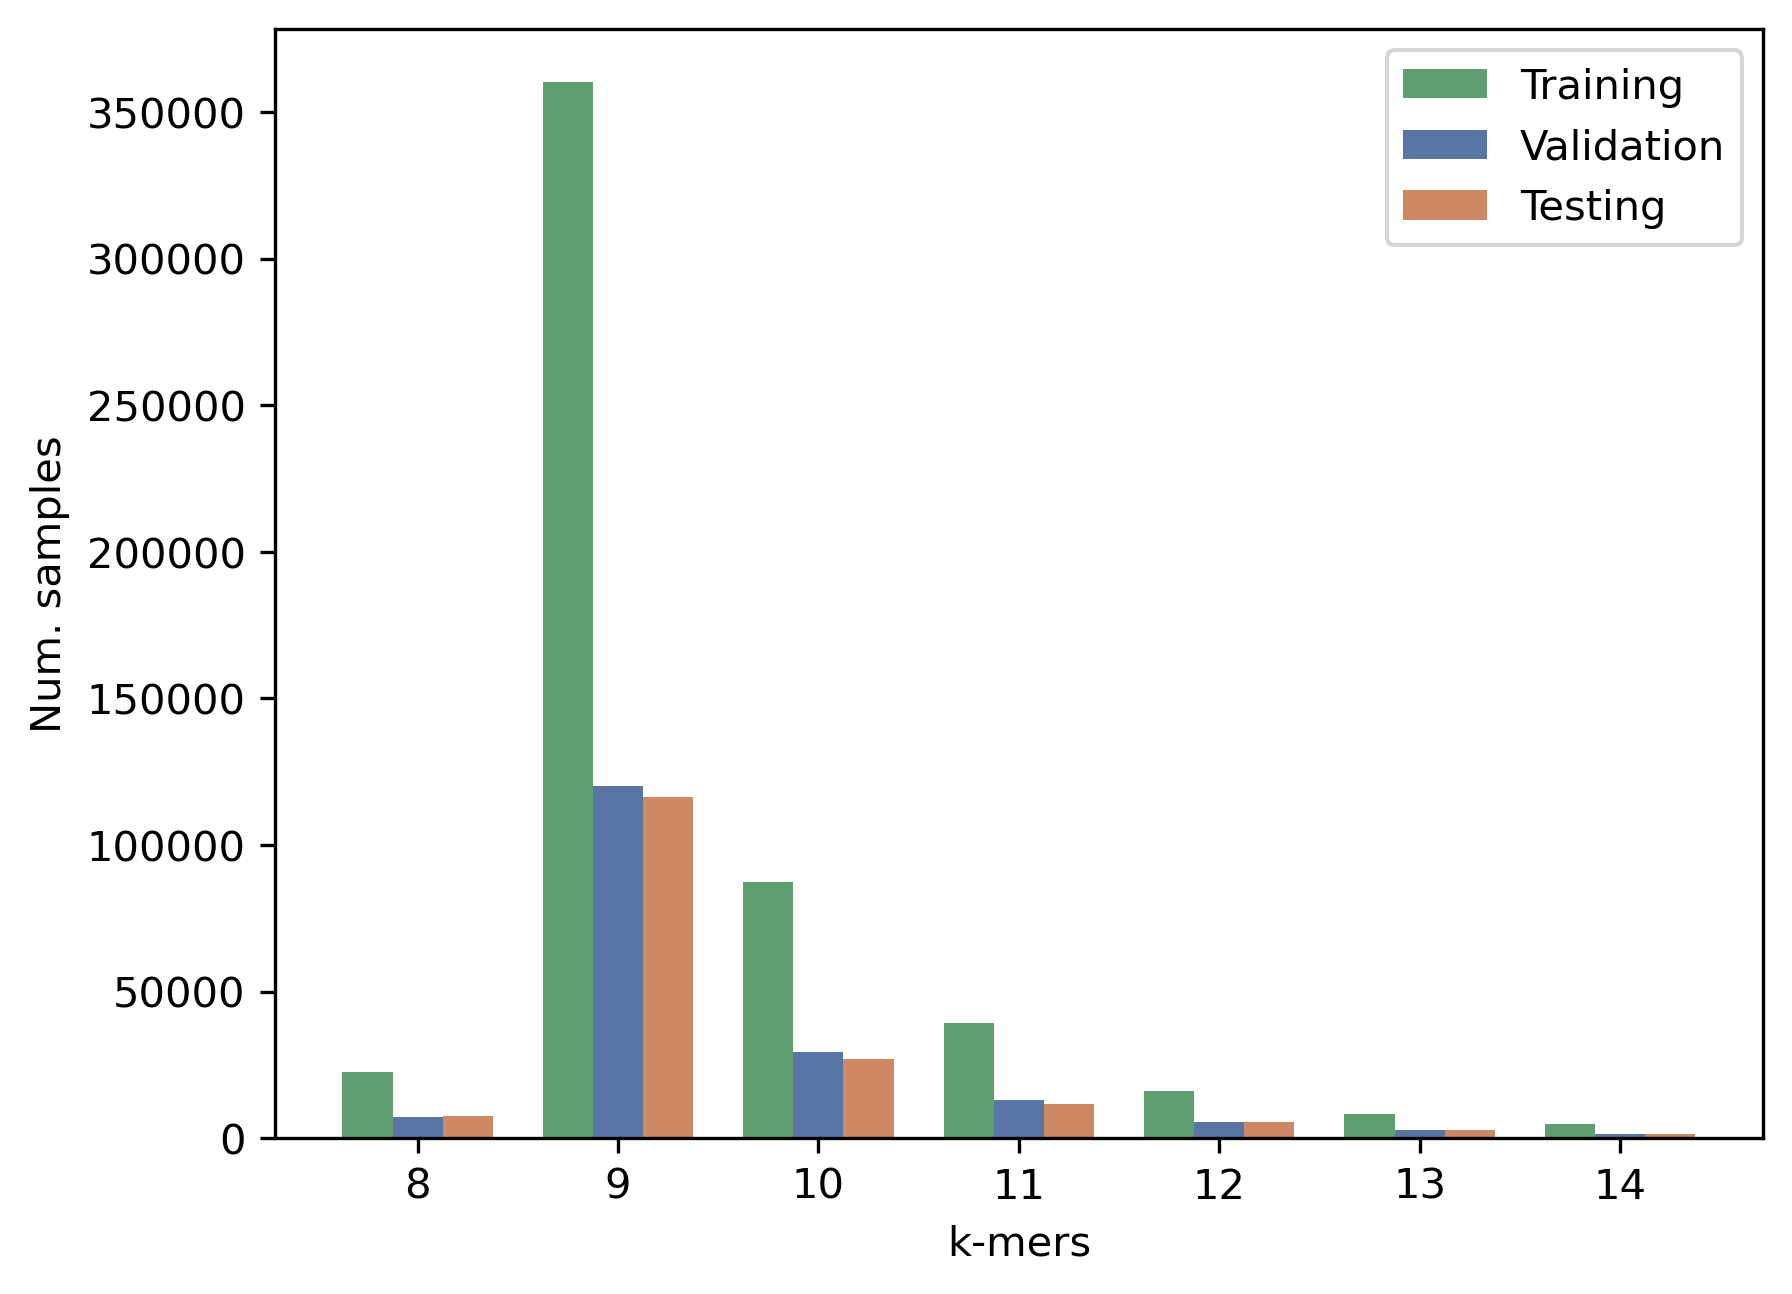
\includegraphics[width=0.8\textwidth]{img/proposal/dataset_samples}
	\caption{
		Cuantificación de las muestras por \textit{k-mers} dentro de los conjuntos de entrenamiento, validación y pruebas. El conjunto de datos se obtuvo de Anthem \cite{mei2021anthem}.}
	\label{fig:samples}
\end{figure}


\section{\textit{Transformer} pre-entrenados}

Evaluamos seis modelos de transformadores: TAPE \citep{rao2019evaluating}, ProtBert-BFD \citep{elnaggar2021prottrans} y ESM2 \citep{lin2023evolutionary} (ESM2(t6), ESM2(t12), ESM2(t30), ESM2(t33)). Estos modelos fueron entrenados con grandes conjuntos de datos de secuencias de proteínas como Pfam \citep{el2019pfam},  BFD y UniRef50 \citep{suzek2015uniref}. Además, se realizo \textit{fine-tuning } para la predicción de unión pMHC-I. En la Tabla \ref{tab:pretrained}, presentamos las características de cada modelo.

\begin{table}[t]%
	\centering
	\caption{Diferencias significativas entre los modelos TAPE, ProtBert-DFB y ESM2. HS: \textit{Hidden size}; AH: \textit{Attention heads}.}
	\label{tab:pretrained}%
	\setlength{\tabcolsep}{0.5em} % for the horizontal padding
	{\renewcommand{\arraystretch}{1.5}% for the vertical padding
	\begin{tabular}{llrrrrr}
		
		\textbf{Modelo}   & \textbf{BD} & \textbf{Muestras} & \textbf{Capas} & \textbf{HS} & \textbf{AH} & \textbf{Params.} \\
		\midrule
		TAPE             & Pfam             & 30M                   & 12              & 768                  & 12                       & 92M                 \\
		ProtBert-BFD     & BFD              & 2122M                 & 30              & 1024                 & 16                       & 420M                \\
		ESM2(t6)  & Uniref50         & 60M                   & 6               & 320                  & 20                       & 8M                  \\
		ESM2(t12)  & Uniref50         & 60M                   & 12              & 480                  & 20                       & 35M                 \\
		ESM2(t30) & Uniref50         & 60M                   & 30              & 640                  & 20                       & 150M                \\
		ESM2(t33)  & Uniref50         & 60M                   & 33              & 1280                 & 20                       & 650M               \\
		
	\end{tabular}}
	
\end{table}

\subsection{TAPE}


\textit{Tasks Assessing Protein Embeddings} (TAPE) \citep{rao2019evaluating} es el primer intento de evaluar el aprendizaje semi-supervisado en secuencias de proteínas. TAPE consta de doce capas de 512 unidades con ocho \textit{attention-heads}, lo que resulta en un total de 92 millones de parámetros. Los autores aplicaron entrenamiento semi-supervisado con la base de datos Pfam \citep{el2019pfam}, que contiene treinta millones de dominios de proteínas. Además, el conjunto de datos Pfam representa un subconjunto del \textit{Knowledge Base UniProt} (UniProtKB) \citep{uniprot2018uniprot}; en particular, Pfam utilizó secuencias de \textit{Reference Proteomes} \citep{finn2016pfam} en lugar de utilizar todo el conjunto de datos de UniProtKB. En consecuencia, Pfam tiene casi la mitad de las secuencias de proteínas que otras bases de datos extraídas de UniProtKB.

\subsection{ProtBert-BFD}

ProtBert-BFD es parte de una familia de modelos de ProtTrans \citep{elnaggar2021prottrans}. Los autores evaluaron varias arquitecturas de aprendizaje profundo con los conjuntos de datos BFD, UniRef50 y UniRef100, cada uno con 2122, 45 y 216 millones de secuencias. Añadido a esto, BFD se considera la colección más extensa de secuencias de proteínas; fusiona UniProt \citep{uniprot2019uniprot} y proteínas de múltiples proyectos de secuenciación de metagenómica. Mientras tanto, UniRef \citep{suzek2015uniref} proporciona un conjunto \textit{clusterized} de secuencias de proteínas de UniProtKB. Es importante destacar que el conjunto de datos más grande, BFD, las muestras tienen ruido y contiene errores en las secuencias \citep{elnaggar2021prottrans}.

Algunos de los modelos propuestos son ProtBert-BFD, ProtT5-XL y ProtT5-XXL, que tienen 420 millones, 3 mil millones y 11 mil millones de parámetros, respectivamente. ProtBert-BFD se entrenó con BFD; mientras tanto, los modelos ProtT5 se entrenaron inicialmente con BFD y luego con UniRef50, lo que mejoró el rendimiento en un 2.8\% y un 1.4\% para ProtT5-XL y ProtT5-XXL, respectivamente. Sin embargo, ProtT5-XL superó tanto a ProtBert-BFD como al modelo más grande, ProtT5-XXL. Los autores afirmaron que la cantidad de muestras mejoraba el rendimiento, pero no observaron una similitud consistente con el tamaño del modelo. Sugerían que modelos más grandes ven menos muestras con la misma potencia de cálculo, por lo que los modelos más grandes necesitan conjuntos de datos más grandes. Por esta razón, hemos optado por ProtBert, ya que es más pequeño que ProtT5-XL y creemos que se adapta mejor al tamaño del conjunto de datos actual para esta investigación.

\subsection{ESM2}


ESM-2 \citep{lin2023evolutionary} es una familia de modelos \textit{Transformer} que tienen  desde 8 millones hasta 15 billones de parámetros. El modelo se basa en BERT \citep{devlin2018bert} y supera a su versión anterior, ESM-1b \citep{rives2021biological}, al eliminar las capas de \textit{dropout} en las capas ocultas y de atención. Además, los autores sugirieron que los métodos de codificación de posición absoluta no se extrapolan bien; en consecuencia, utilizaron la \textit{Rotary Position Embedding} (RoPE). Significativamente, el uso de RoPE aumenta ligeramente el costo de entrenamiento; al mismo tiempo, mejora la calidad del modelo para modelos pequeños \citep{lin2023evolutionary}. Además, los autores utilizaron el conjunto de datos no redundante UniRef50 \citep{suzek2015uniref} de UniProt, que contiene 60 millones de secuencias de proteínas.


\section{\textit{Fine-tuning}}\label{sec:fine-tuned}

Una manera de realizar \textit{transfer learning} de modelos de \textit{deep learning} grandes, es realizando \textit{fine-tuning}. Está metodología, generalmente se aplica cuando tenemos un modelo entrenado con una base de datos muy grande, como por ejemplo una base de datos de texto de todas las páginas de internet. Luego, queremos adaptar dicho modelo para una tarea específica y en donde no contamos una base de datos muy grande, como por ejemplo un conjunto de muetras de análisis de sentimientos; entonces, podemos aplicar \textit{fine-tuning} al modelo entrenado con todo el texto de internet para una nueva tarea, entrenandolo de nuevo pero esta vez con el objetivo de predecir el sentimiento de un texto. En resumen está técnica consiste en modificar las ultimas capas del modelo pre-entrenado. La modificación puede ser eliminando las ultimas capas y agregando capas lineales, convoluciones, o recurrentes. Luego, se vuelve a entrenar el modelo una vez mas con el objetivo que el modelo se adapte al nuevo problema. En la Figura \ref{fig:fine-tuning}, mostramos un ejemplo de este procedimiento.

Luego, se sabe que al entrenar modelos de \textit{Transformers} grandes, las capas finales experimentan cambios más significativos, mientras que las capas iniciales, más cercanas a la entrada, sufren modificaciones relativamente menores. En otras palabras, las ultimas capas son mas específicas, mientras que las capas iniciales, representan caraterísticas generales del problema \citep{merchant2020happens,lee2019would,kovaleva2019revealing}. Debido a esto, es comun en los procesos de f\textit{ine-tuning}, eliminar las ultimas capas y agregar otras capas al final del modelo. En este trabajo,  apilamos en cascada un bloque BiLSTM al final del modelo pre-entrenado (ver Figura \ref{fig:fine-tuning_proposal}), luego se agrego una capa lineal con dos neuronas como salida para el problema de clasificación pMHC. Finalmente, este modelo se entreno con una base de datos de muestras de pMHC. Las características de los modelos BERT pre-entrenados se detallan en la Tabla \ref{tab:pretrained} mientras que las características del bloque LSTM utilizado en el proceso de \textit{fine-tuning} fueron inspirados por el trabajo de \cite{zhang2022hlab} y se detallan en la Tabla \ref{tab:biLSTM}.

 



\begin{figure}[H]
	\centering
	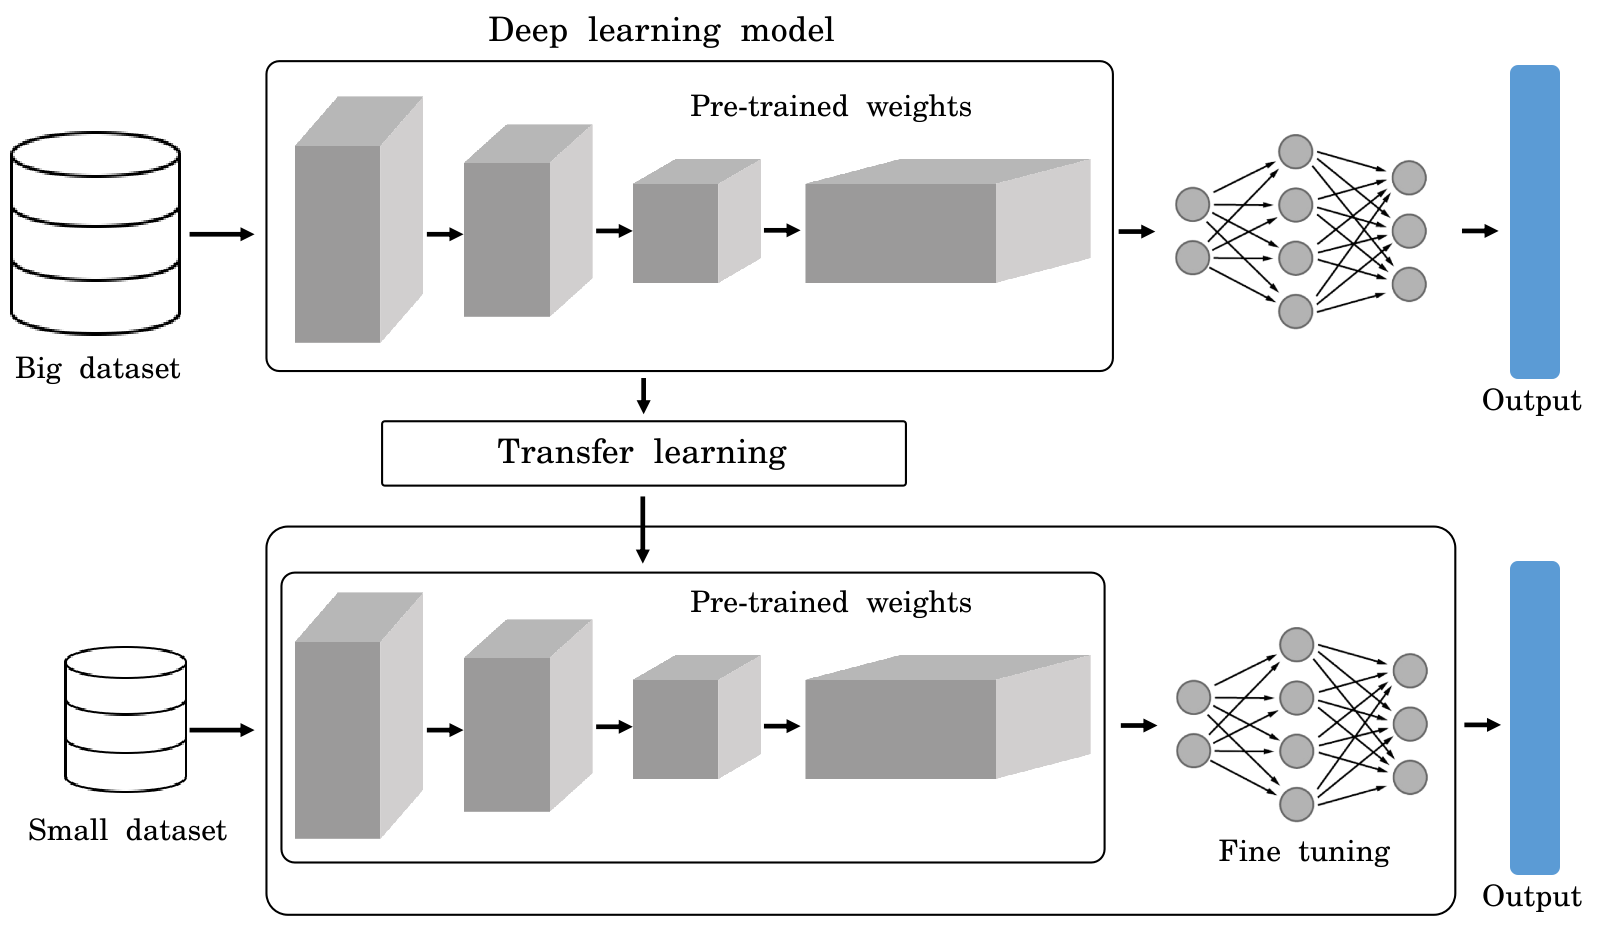
\includegraphics[width=\textwidth]{../img/proposal/fine_tuning}	
	\caption[Ejemplo de aplicación de \textit{Fine-tuning}]{Ejemplo de aplicación de \textit{Fine-tuning}. Primero, se entrena un modelo para una tarea $x$ con una gran base de datos, luego puede aprovecharse ese aprendizaje para otra tarea similar $y$ que no tenga una base de datos grande. Generalmente, en este proceso, se eliminan las ultimas capas y se agregan otras capas lineales, convoluciones o recurrentes. Fuente: Adaptado de  \cite{prince2023understanding}.}		
	\label{fig:fine-tuning}
\end{figure}


\begin{figure}[H]
	\centering
	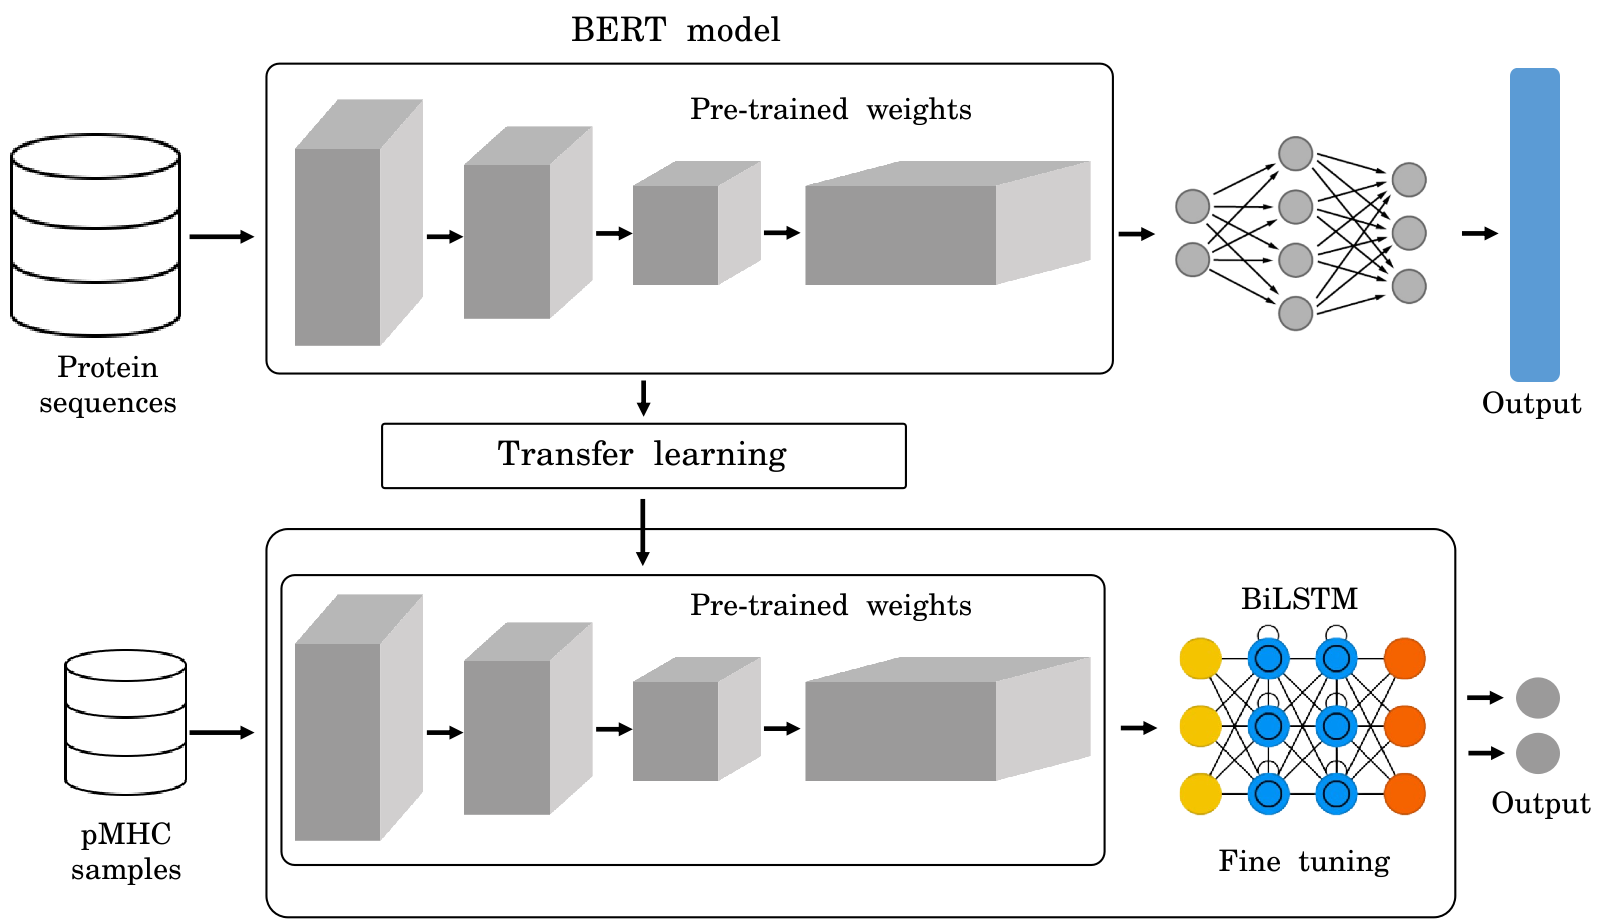
\includegraphics[width=\textwidth]{../img/proposal/fine_tuning_proposal}	
	\caption[Fine-tuning al modelo BERT]{\textit{Fine-tuning} propuesto. Se toma las primeras capas de un modelo BERT pre-entrenado con bases de datos de secuencias de proteínas. Luego, se agrega un bloque de capas BiLSTM al final y se entrena de nuevo con una base de datos pequeña de muestras pMHC. Fuente: Adaptado de  \cite{prince2023understanding}.}		
	\label{fig:fine-tuning_proposal}
\end{figure}
% agregar una figura especifica del finetuning




\begin{table}[t]%
	\centering
	\caption{Características del bloque BiLSTM utilizado en el \textit{fine-tuning}.}
	\label{tab:biLSTM}%
	\setlength{\tabcolsep}{0.5em} % for the horizontal padding
	{\renewcommand{\arraystretch}{1.5}% for the vertical padding
		\begin{tabular}{lp{9cm}p{1cm}p{1cm}}
			\hline
			\textbf{Tipo}   & \textbf{Entada} & \textbf{Salida}& \textbf{Capas} \\ \hline
			
			BiLSTM & Salida del modelo BERT (Tabla \ref{tab:pretrained}, columna HS) & 768 & 2 \\
			
			Dropout & 0.1\% & - & - \\
			Lineal & 1536 & 2 & 1 \\ \hline
	\end{tabular}}
	
\end{table}



\section{\textit{Gradient Accumulation Steps}}\label{sec:gas}

Adicionalmente, los modelos de \textit{Transformer} grandes utilizan bastante memoria de la GPU. Por lo tanto, inspirados en trabajos similares sobre entrenamiento de modelos grandes de \textit{Transformers} para problemas de NLP \citep{anil2021large,zhang2023adam,huang2023measuring}, evaluamos los resultados de aplicar \textit{Gradient Accumulation Steps} durante el entrenamiento. El proceso se explica en la Figura \ref{fig:gas_example}, por ejemplo en un entrenamiento normal durante el proceso de actualización de parámetros en el algoritmo de aprendizaje, se considera un solo \textit{mini-batch} para obtener las gradientes y luego actualiza los parametros; mientras que en el enfoque utilizando \textit{Gradient Accumulation Steps}, se consideran varios \textit{mini-batchs}, se suman sus gradientes y luego estas gradientes acumuladas son utilizadas para actualizar los parámetros.



\begin{figure}[H]
	\centering
	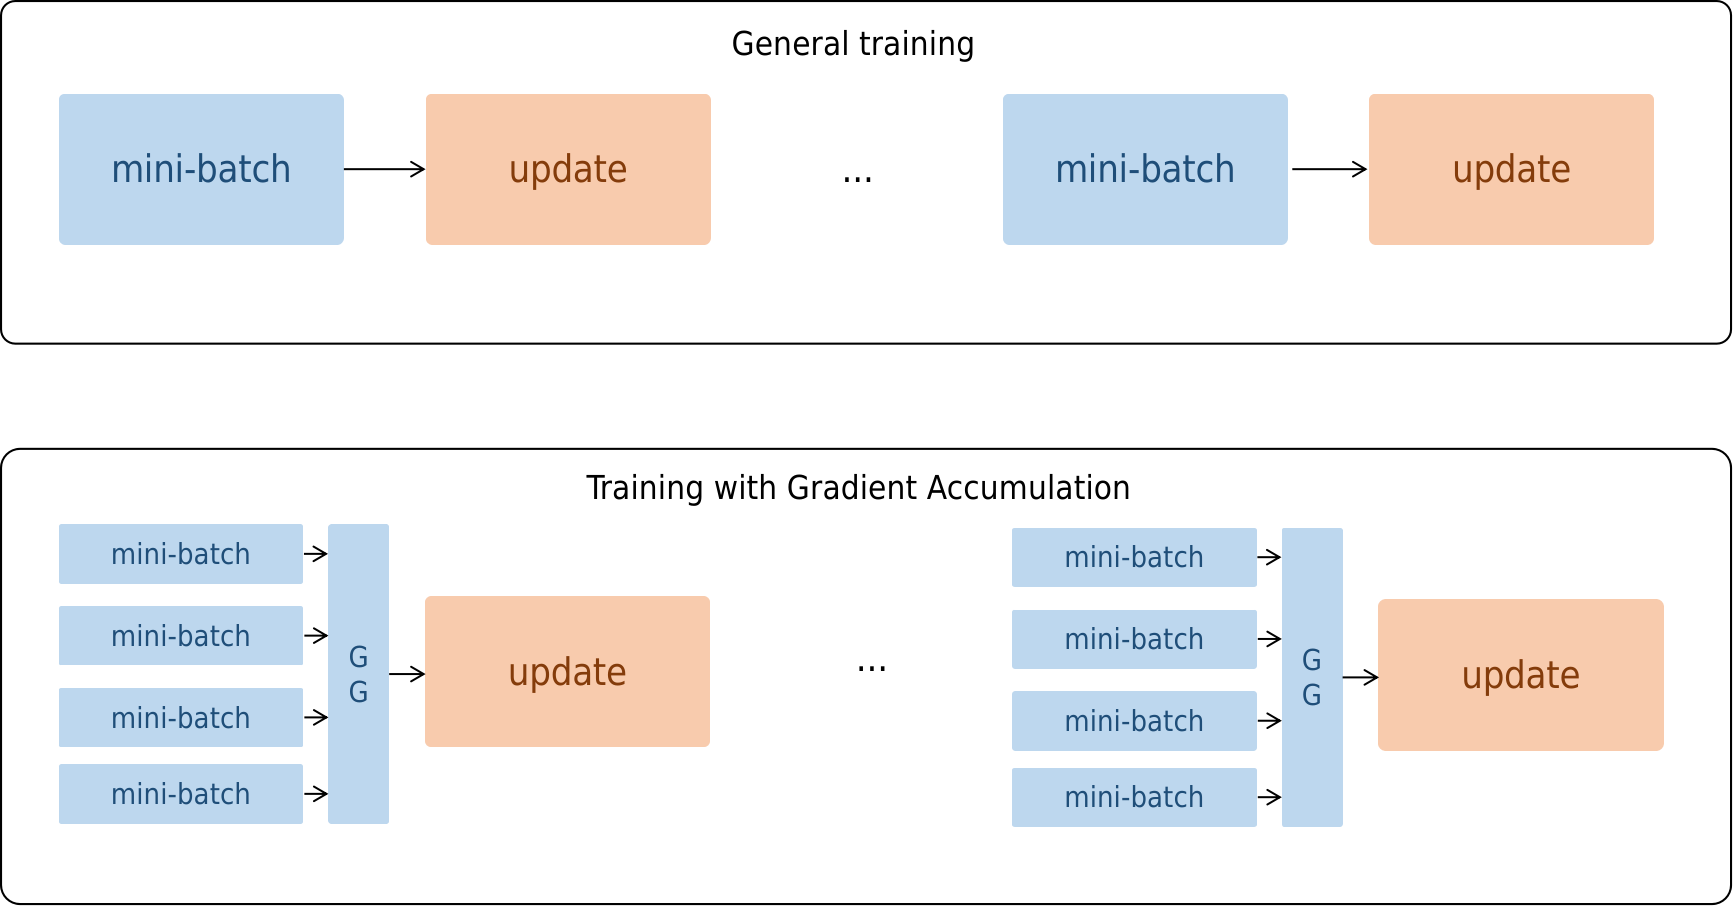
\includegraphics[width=\textwidth]{../img/proposal/gas_own}	
	\caption[Ejemplo de aplicación de \textit{Gradient Accumulation Steps}]{Ejemplo de aplicación de \textit{Gradient Accumulation Steps} durante el entranamiento de modelos de Deep Learning. En este caso, un entrenamiento general considera un solo \textit{mini-batch} para obtener las gradientes y luego actualiza los parámetros; mientras que en el enfoque utilizando \textit{Gradient Accumulation Steps}, se consideran varios \textit{mini-batchs}, se suman sus gradientes, luego estas gradientes acumuladas son utilizadas para actualizar los parámetros.  Fuente: Adaptado de  \cite{prince2023understanding}.}		
	\label{fig:gas_example}
\end{figure}



\section{Hiperparámetros}\label{sec:hyperparam}
Finalmente, utilizamos los siguientes hiperparámetros: tasa de aprendizaje de 5e-5, \textit{weight decay} de 0.0001, \textit{momentum} de 0.9, \textit{warn-up steps} de 1000 con \textit{linear decay}, optimizador ADAM ($\beta_1 = 0.9, \beta_2=0.999$) y \textit{early stopping}. Estos valores fueron utilizados por BERTMHC \citep{cheng2021bertmhc} después de buscar los mejores parámetros utilizando \textit{grid search}.

\section{Ambiente de trabajo}

Para entrenar los modelos pequeños de \textit{deep learning}, con menos de 200 millones de parámetros, se utilizo una tarjeta RTX3070, esta cuenta con 8GB de memoria dedicada de vídeo. Para entrenar los modelos grandes, mas de 200 millones de parámetros, se utilizo GPUs en la nube. La plataforma utilizda fue Paperspace, esta brinda diferentes opciones de GPUs, las utilizadas en este proyecto fueron la A100 y la A4000.

\section{Clasificación binaria y Métricas}

El problema de predicción de unión pMHC es un problema de regresión. Sin embargo, basado en el conjunto de datos utilizado en este estudio, también podría abordarse como un problema de clasificación binaria al seleccionar un umbral apropiado. Las métricas de aprendizaje automático utilizadas en este trabajo son: \textit{accuracy, precision, recall, f-1 score, Area Under the Curve (AUC)}, y \textit{Matthews Correlation Coefficient} (MCC). Todas las métricas están descritas en las ecuaciones siguientes.

\begin{equation}\label{equa:acc}
	Accuracy = \frac{TP+TN}{TP+TN+FP+FN}
\end{equation}

\begin{equation}\label{equa:precision}
	Precision = \frac{TP}{TP+FP}
\end{equation}

\begin{equation}\label{equa:recall}
	Sensitivity = Recall = \frac{TP}{TP+FN}
\end{equation}

\begin{equation}\label{equa:f1}
	F1 = \frac{2*Precision*Recall}{Precision+Recall} = \frac{2 \times TP}{2*TP+FP+FN}
\end{equation}


\begin{equation}\label{equa:FPR}
	Specificity = \frac{TN}{FP+TN}
\end{equation}

\begin{equation}\label{equa:MCC}
	MCC = \frac{TP \times TN - FP \times FN}{ \sqrt{ (TP+FP)(TP  + FN)(TN+FP)(TN+FN)}  }
\end{equation}

donde \textit{TP}, hace referencia a la cantidad de muestras que eran verdaderas y han sido reconocidas como verdaderas; \textit{TN}, hace referencia a la cantidad de muestras que eran verdaderas y han sido reconocidas como falsas; \textit{FP}, son las muestras que eran falsas, pero fueron reconocidas como verdaderas; \textit{FN}, son las muestras que eran falsas y fueron reconocidas como falsas.
